\documentclass[a4paper 12pts]{article}
\usepackage[utf8]{inputenc}
\usepackage[T1]{fontenc}
\usepackage[francais]{babel}
\usepackage{graphicx}
\usepackage{verbatim}
\usepackage{hyperref}

%macro



\usepackage[T1]{fontenc}
\usepackage{fancyvrb}
\usepackage{xcolor}

\definecolor{Zgris}{rgb}{0.87,0.85,0.85}

\newsavebox{\BBbox}
\newenvironment{DDbox}[1]{
\begin{lrbox}{\BBbox}\begin{minipage}{\linewidth}}
{\end{minipage}\end{lrbox}\noindent\colorbox{Zgris}{\usebox{\BBbox}} \\
[.5cm]}



\title{Manuel Utilisateur iRover}

\author{R. Joachim CLAYTON}

\begin{document}

\maketitle


\begin{figure}[h]
   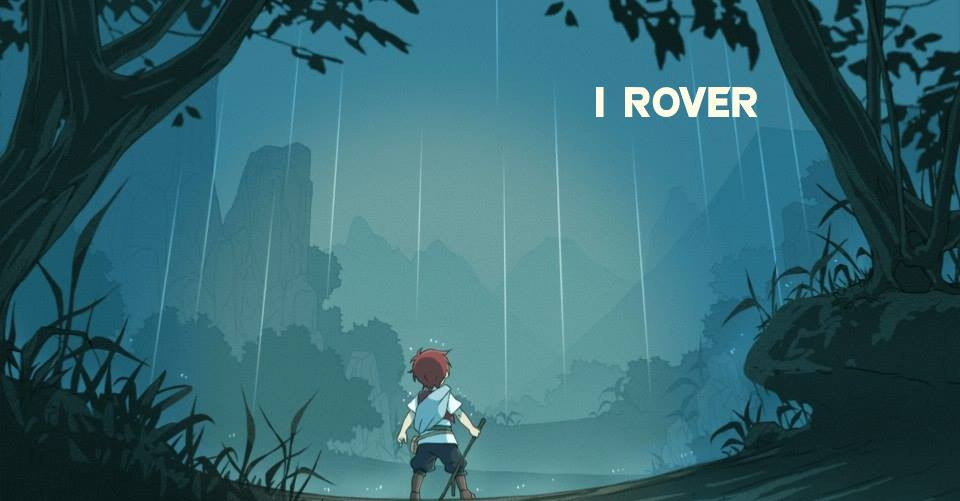
\includegraphics[width=350pt]{Illustration/proj_irover.jpg}
	\caption{iRover, l'histoire d'un héros qu'on appellait Robot}
\end{figure}



\newpage


\renewcommand{\contentsname}{Sommaire} 
\tableofcontents

\newpage



\section{iRover, l'histoire d'un héros}

%background, histoire, scénario

\vspace{1cm}

Cette partie est dédiée à l'histoire de notre héros, son monde et ses motivations.
Si vous désirez en apprendre plus, laissez-moi vous conter son histoire.

\vspace{1cm}

\subsection{Le monde de Lorr}

\vspace{1cm}

\begin{figure}[h]
	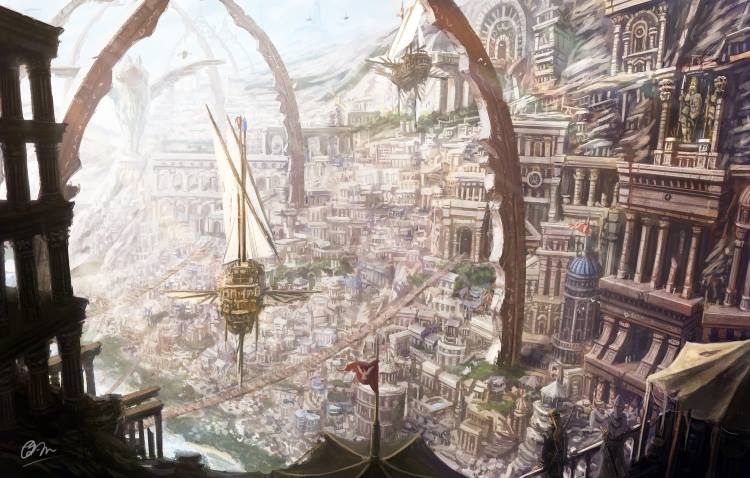
\includegraphics[width=350pt, height=180pt]{Illustration/Lina.jpg}
	\caption{Lina}
\end{figure}

\vspace{1cm}

Le pays de Lorr, vaste étendue de terre fertile entourée de montagnes et de forêts luxuriantes, abrite la vallée perdue du Vertou, 
là où nul n'a mis les pieds depuis plusieurs siècles.\\
On raconte que c'est ici que le grand pirate du nom de Stevy J. y aurait caché un trésor :"le chamallow magique".\\
Notre héros, intrépide aventurier du nom de Rover quitte alors sa ville natale Lina, où l'industrie et la maitrise de l'acier règne, et part à la recherche de cette sucrerie antique.\\

\newpage

Cependant, cette mystérieuse vallée est habitée par d'étranges créatures : "des chou-kêtes".\\
Une horde de monstres farouchement attachées à leur territoire, connue pour attaquer quiconque y pénetrera.\\

\vspace{1cm}

\begin{figure}[h]
	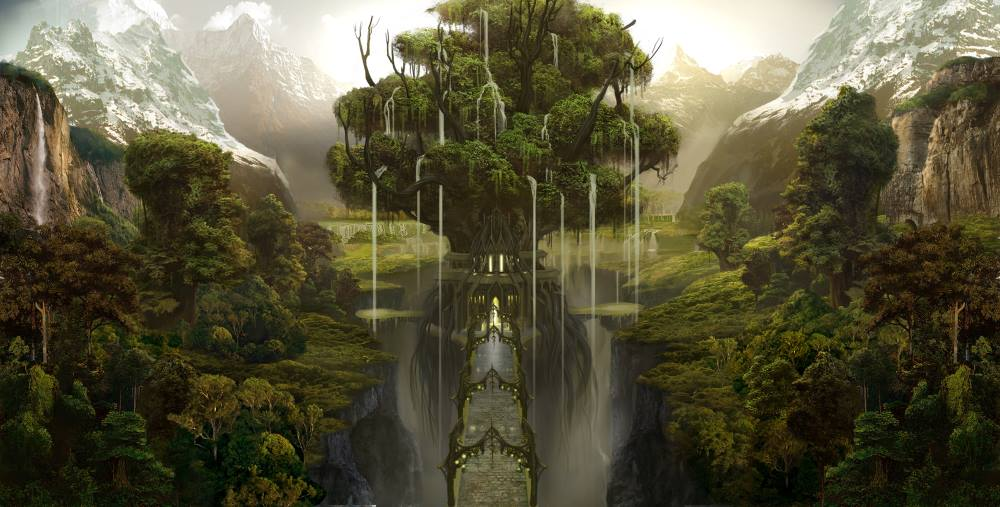
\includegraphics[width=350pt]{Illustration/Vertou.jpg}
	\caption{Vertou}
\end{figure}



\vspace{1cm}


\newpage
\subsection{Stevy J.}

\vspace{1cm}

\begin{figure}[h]
  	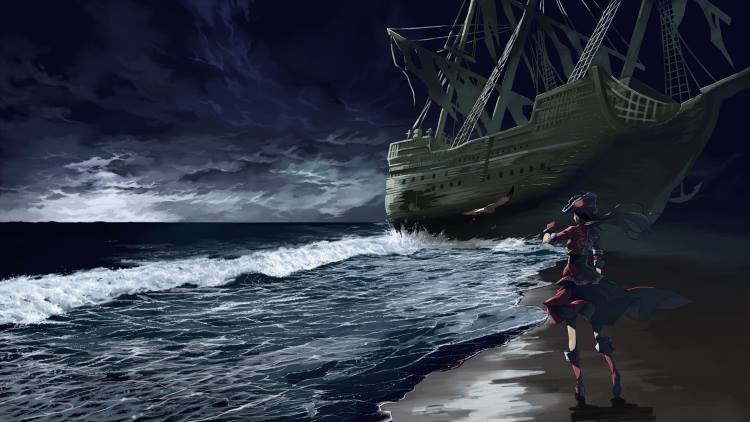
\includegraphics[width=350pt]{Illustration/Steve.jpg}
	\caption{Illustration du bateau de Steve}
\end{figure}

\vspace{1cm}

A une époque lointaine, Steven Joseph Obs de son nom complet, grand pirate et chasseur de trésors, écuma les 8 océans du monde pour venir finir ses jours dans le pays de Lorr.\\
On raconte qu'il aurait réussi à trouver le chamallow magique, un artefact qui apporterait gloire, richesse et sucrerie infinie à quiconque le possèdera.\\
Stevy sera capturé et pendu pour piraterie et ne révèlera jamais ses secrets même dans sa biographie post-mortem.\\
Beaucoup d'aventuriers ont tenté de retrouver son trésor partout dans le monde mais il n'existe qu'un seul endroit où personne n'a mis les pieds après le passage du celèbre pirate.



\newpage

\subsection{Rover, un héros pas comme les autres}

\vspace{1cm}

\begin{figure}[h]
  	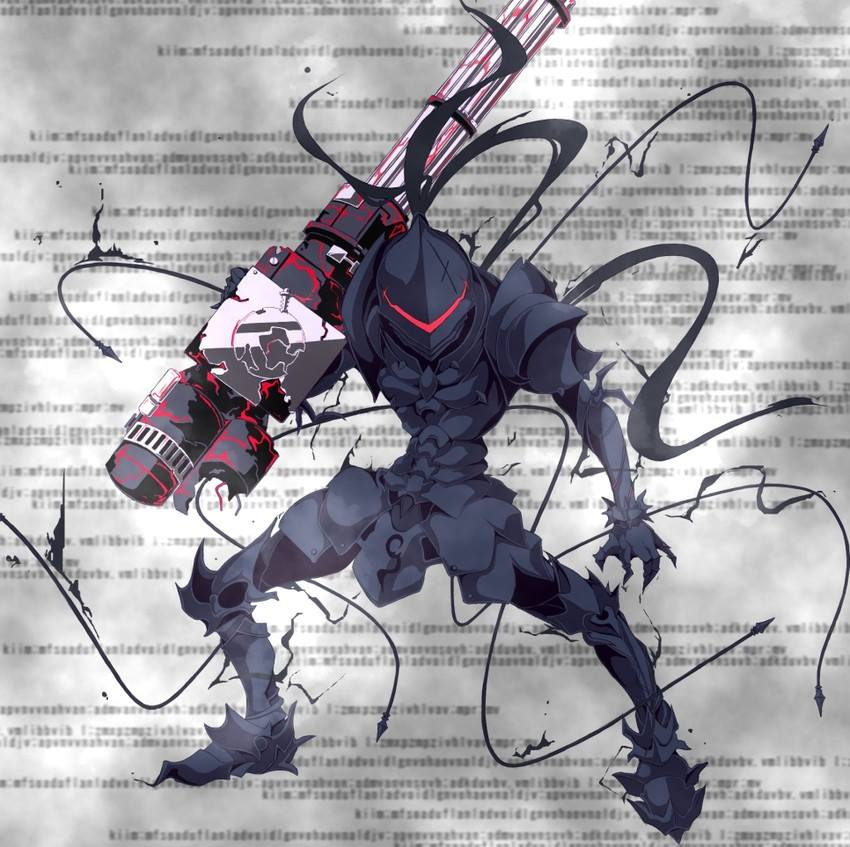
\includegraphics[width=350pt]{Illustration/Rover.jpg}
	\caption{Rover en Armure}
\end{figure}


Rover, notre héros, un apprenti forgeron, rêve d'aventure ! Ses années d'apprentissage lui permirent de créer une armure lui donnant une apparance de robot et surtout augmentant sa protection contre les dangers de la vie au quotidien.
Lors de ses excursions il ne sort jamais sans son arme : un petit bazooka, une arme de poing d'une très grande puissance.


\subsection{Les Chou-kêtes}
\vspace{1cm}


\begin{figure}[h]
  	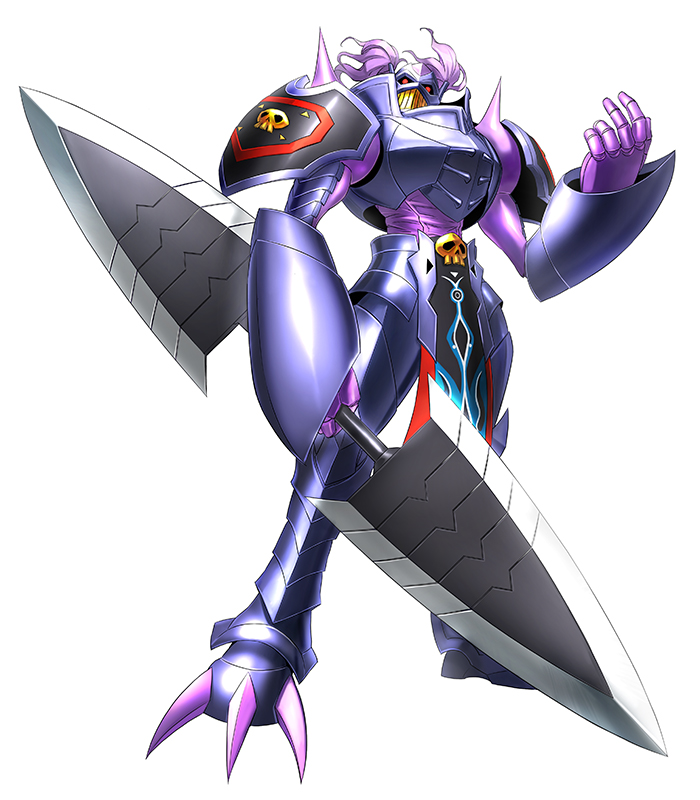
\includegraphics[width=300pt]{Illustration/Badboy.jpg}
	\caption{Général des Chou-Kêtes}
\end{figure}

\vspace{0.8 cm}

Bien des sciècles après la mort de Stevy J., on raconte que des créatures marines surgirent des océans pour venir habiter dans la vallée.
Personne ne sait exactement qui ils sont, ni d'ou ils viennent. Le dialogue avec ces êtres est impossible et il ne répondent que par la violence aux étrangers qui
pénetrent sur leur territoire.



%regle du jeu

\section{But du jeu}


\vspace{2cm}

L'objectif principal du jeu (ou plutot de notre jeune ami) est de ramasser tous les trésors présents 
sur le terrain afin d'atteindre gloire et richesse et surtout un jour trouver le chamallow magique.\\

Des coffres seront disséminés sur la carte, souvent derrière des obstacles que le héros devra contourner.\\ 
Des ennemis (les chou-kêtes) pourront également attaquer notre héros et donc un combat sans merci s'enclenchera entre héros et monstre.\\


\begin{figure}[h]
   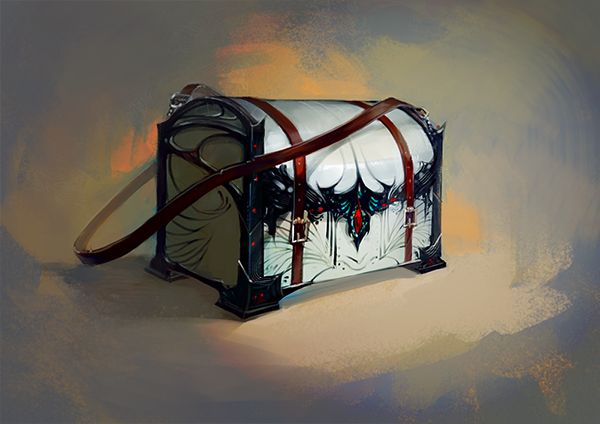
\includegraphics[width=350pt]{Illustration/coffre.jpg}
\caption{coffre au trésor}
\end{figure}


Le jeu prendra fin une fois tous les coffres ramassés ou si notre héros ne peut plus continuer son aventure.




\newpage

\section{Manuel d'installation}

\vspace{1.5cm}


\subsection{makefile}


Cette partie est dédiée à l'installation de l'application.
Depuis un terminal linux.
Mettez vous dans le dossier courrant où les fichiers de l'application sont présents puis tappez :
Makefile.

%graaaaahhhhhhhhh il devrait y avoir plus d'info....

\subsection{Génération Doc Doxygen}

executer la commande pour générer le fichier de config

\vspace{0.5 cm}
\begin{DDbox}{\linewidth}
\begin{verbatim}
doxygen -g config_dox
\end{verbatim}
\end{DDbox}


modifier les champs suivants dans le fichier de config :

\vspace{0.3 cm}


\begin{DDbox}{\linewidth}
\begin{verbatim}


PROJECT_NAME           = "I-rover"

PROJECT_NUMBER         = 1.0

OUTPUT_LANGUAGE        = French
INPUT                  = CodeMain

FILE_PATTERNS          = *.hpp *.cpp


\end{verbatim}
\end{DDbox}


executer la commande :

\vspace{0.3 cm}

\begin{DDbox}{\linewidth}
\begin{verbatim}

doxygen config\_dox
\end{verbatim}
\end{DDbox}
\vspace{0.3 cm}

\newpage

\section{Documentation utilisateur}

%documentation utilisateur : donner des informations à des utilisateurs lambda sans grande connaissance informatique, avec des mots simple sur le fonctionnement de l'application.
%donner egalement une description simple de comment est faite ou est géré les partie de l'application.

\vspace{2cm}

Cette partie est dédiée aux utilisateurs recherchant à comprendre les mécanismes de cette application.
Si vous recherchez des détails techniques, merci de vous reférer au Manuel Technique ou à la Doxygen du projet.
Nous vous expliquerons ici comment les divers éléments du jeu s'articulent afin de vous permettre une meilleure expérience utilisateur.

\vspace{0.5cm}	

\subsection{Les personnages}

\vspace{1cm}


Le jeu possède deux types de personnage : 

\vspace{0.5cm}

\begin{enumerate}
	\item Le héros, notre rover ou petit robot
	\item Les ennemis, les chou-kêtes.
\end{enumerate}

\vspace{0.5cm}

Ces deux types de personnage peuvent à la fois :

\vspace{0.5cm}

\begin{enumerate}
	\item se déplacer, avancer case par case 
	\item combattre, lancer un combat
\end{enumerate}

\vspace{0.5cm}

Chaque personnage possède des coordonnées indiquant son emplacement en temps réel sur la carte ainsi que des statistiques propres à chacun mais aussi possèdera une armure ainsi qu'une arme.

\newpage
\subsubsection{Le robot, Rover}
\vspace{1cm}

Le robot se déplace sur la carte case par case et rencontrera des obstacles.
N'ayant pas appris à nager et dû à des crises de vertiges récurrentes, il ne pourra ni se déplacer sur l'eau ni grimper sur les rochers,
les arbres, les murs et même les buissons !

Le robot, en plus de pouvoir se déplacer sur le terrain, peut aussi ramasser des clefs et ouvrir des coffres.
Pour cela, le robot possède un inventaire représenté par le nombre de clefs que possède le robot.\\
Lorsque le robot va ramasser une clef, le nombre de clefs que le robot possède augmente donc de 1.\\
Inversement, lorsque notre robot ouvrira un coffre, le nombre de clefs dont il dispose diminura de 1 tout en sachant qu'il n'arrivera pas à ouvrir un coffre sans clef.\\
Le robot devra également combattre les ennemis pour rester en vie s'il a le malheur de croiser un chou-kête.\\
Il possède une armure et une arme.
Le robot peut également prendre connaissance de ce qui l'entoure grâce à sa vision et ses senseurs. Il sait donc où aller et quoi faire.

\vspace{0.75cm}

\subsubsection{Les ennemis}


Certains ennemis seront présents sur le terrain et mettront le robot en difficulté. 
Le robot devra alors combattre ces ennemis s'il les rencontre afin de rester en vie.

Lorsque le robot se trouve à côté d'un ennemi, il est obligé de le combattre. 
Une fois l'ennemi vaincu, celui-ci disparaît du terrain mais dans le cas contraire, 
notre héros ne sera plus en mesure de continuer et le jeu prendra fin.
Les ennemis tout comme le héros peuvent se déplacer sur la carte mais ils auront un déplacement différent par rapport au héros.



\newpage
\subsection{Les coffres}


\vspace{0.75cm}

Les coffres sont des éléments posé aléatoirement sur la carte. Ils possèdent des trésors que notre héros souhaite récupérer.
Ils ne peuvent s'ouvrir qu'à l'aide de clefs.


\vspace{0.75cm}

\subsection{Les clefs}

\vspace{0.75cm}

Les clefs sont des éléments posé aléatoirement sur la carte. Ils permettent d'ouvrir les coffres au trésor disséminé un peu partout sur la carte.\\
Les clefs se détériore après leur utilisation fesant d'eux un consomable.


\vspace{0.75cm}


\subsection{L'environnement}
La carte sur laquelle le robot se déplace est construite à l'aide de Tiled, un logiciel permettant de créer des cartes case par case. 
Pour les cartes modélisées, on distingue deux types de cases:


\vspace{0.75cm}

La carte sur laquelle le robot se déplace est constitué de cases comme appelles comunémant des Tiles (carreaux). \\
On distingue deux types de cases:

\begin{enumerate}
	\item Les cases où le robot peut se déplacer.
	\item Les cases où le robot ne peut pas se déplacer.
\end{enumerate}

Ces cases permettent de décrire le décor et le type de terrain où se balade notre robot.
L'environnement sert de base également pour la disposition des autres éléments tel que les coffres, les clefs, et ennemis.\\
La rencontre avec un de ces éléments entraine une gestion d'évênements.

L'environnement servira de base également pour la disposition des autres entités présentes (coffre, clef, ennemis).
Ceux-ci sont disposés aléatoirement sur la carte à des endroits accessibles par le héros mais ils ne peuvent pas se déplacer.
La rencontre avec un de ces éléments entraine la gestion des évènements.



\newpage
\subsection{La gestion des évènements}

Le robot, Rover, devra faire face à beaucoup d'évènements : ouvrir un coffre, se battre contre un ennemi, ramasser une clef, se cogner contre un mur etc..
Tout ceci est géré par le comportement de chaque objet mais aussi pour sa hierarchie sur la carte.
Par exemple il doit être possible de marcher sur une clef pour la ramasser alors qu'il doit être impossible de marcher sur un ennemis

\subsubsection {Rencontre avec un ennemi} 
Un ennemi et le héros devront avoir la même importance physique : il ne peuvent pas se superposer.
Un ennemi et le héros n'auront besoin que d'un regard pour enclencher le combat ! 1 case de différence.

\begin{figure}[h!]
	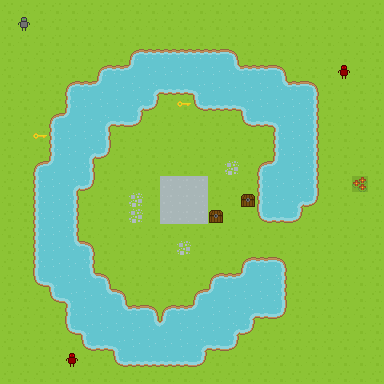
\includegraphics[width=200pt]{Illustration/screens/screen4.png}
\caption{screenshot de la carte numéros 2}
\end{figure}
\vspace{0.75cm}

\subsubsection {Ouverture d'un coffre}
Un coffre et le héros n'ont pas la même importance physique : le héros devra pouvoir "marcher" sur le coffre.
Un coffre et le héros devront impérativement être sur la même case pour que le coffre puisse s'ouvrir, et le héros devra avoir une clé pour que cela soit possible.


%mettre un schéma
\vspace{0.75cm}

\subsubsection {Ramasser une clé}

\vspace{0.75cm}
Une clé et le héros n'ont pas la même importance physique : le héros devra pouvoir "marcher" sur la clé.
La clé et le héros devront impérativement être sur la même case pour que la clé puisse être ramassée par lui.
L'inventaire de clé augmentera alors.

%mettre un schéma
\vspace{0.75cm} 
\subsection{L'interface utilisateur}

\newpage

\subsection{IA}

L'intelligence artificielle est dans notre application ce qui détermine le scénario de ce mini jeu.
En effet notre robot se déplace et agit de façon intelligente.
\vspace{0.75cm}

\subsubsection{Le Path Finding}

\vspace{0.75cm}

Le path finding correspond à la capacité du robot à trouver un chemin à suivre pour atteindre un objectif qu'il se fixe.
Par exemple : 

\vspace{0.5cm}

\begin{enumerate}
\item "Je dois retrouver mon ami qui est en bas à droite de la carte"
\item "Je suis au centre de la carte"
\item "Je regarde le chemin le plus simple pour y aller"
\item "Je le suis jusqu'à destination"
\end{enumerate}

\vspace{0.75cm}

\subsubsection{La découverte de la carte}

\vspace{0.75cm}

La découverte de la carte est ce qu'on appelle un senseur.
Meme si notre amis Rover est pixelisé il est doté de sens lui permettant de "voir" ce qui l'entoure et de comprendre son environnement.
Afin d'utiliser le path finding (expliqué au paragraphe précédent) il a besoin de savoir où il est et où il doit se rendre.

\vspace{0.75cm}

\subsection{Les conditions de fin du jeu}

\vspace{0.75cm}

Le jeu se termine selon deux conditions bien distinctes :
Soit le héros n'est plus apte à continuer son aventure après un combat.
Soit le héros a récupéré tous les coffres de la carte et a réussi son objectif.

\newpage

\section{tutoriel}
\vspace{0.55cm}

Lancer l'application !
Ce tutoriel vous permettra de lancer l'application et d'avoir une idée de comment l'application s'articule.

\vspace{0.25cm}
\begin{figure}[h]
   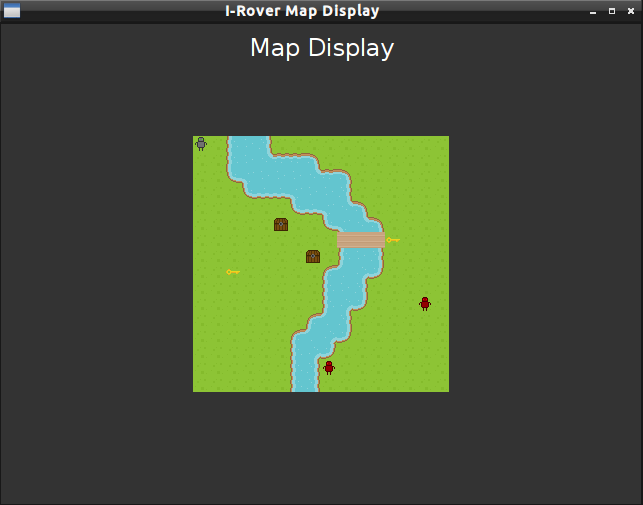
\includegraphics[width=200pt]{Illustration/screens/screen1.png}
	\caption{screenshot de la carte numéro 1}
\end{figure}

Après quelques secondes, notre robot décide d'aller chercher une clef.

\begin{figure}[h]
   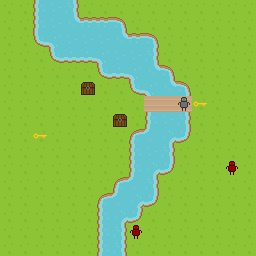
\includegraphics[width=200pt]{Illustration/screens/screen2.png}
\caption{screenshot de Rover proche d'une clef}
\end{figure}

\newpage


Ici nous voyons Rover en mauvaise posture proche d'un ennemi qui l'attaque.

\vspace{1cm}

\begin{figure}[h]   
	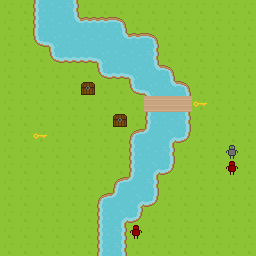
\includegraphics[width=200pt]{Illustration/screens/screen3.png}
\caption{screenshot de Rover proche d'un ennemi}
\end{figure}



\end{document}


